\documentclass[12pt, letterpaper, preprint, comicneue]{aastex63}
%\usepackage[default]{comicneue} % comic sans font for editing
\usepackage[T1]{fontenc}
\usepackage{fontawesome}
\usepackage{color}
\usepackage{amsmath}
\usepackage{natbib}
\usepackage{ctable}
\usepackage{bm}
\usepackage[normalem]{ulem} 
\usepackage{xspace}
\usepackage{paralist}


% typesetting shih
\linespread{1.08} % close to 10/13 spacing
\setlength{\parindent}{1.08\baselineskip} % Bringhurst
\setlength{\parskip}{0ex}
\let\oldbibliography\thebibliography % killin' me.
\renewcommand{\thebibliography}[1]{%
  \oldbibliography{#1}%
  \setlength{\itemsep}{0pt}%
  \setlength{\parsep}{0pt}%
  \setlength{\parskip}{0pt}%
  \setlength{\bibsep}{0ex}
  \raggedright
}
\setlength{\footnotesep}{0ex} % seriously?

% citation alias

% math shih
\newcommand{\setof}[1]{\left\{{#1}\right\}}
\newcommand{\given}{\,|\,}
\newcommand{\lss}{{\small{LSS}}\xspace}

\newcommand{\Om}{\Omega_{\rm m}} 
\newcommand{\Ob}{\Omega_{\rm b}} 
\newcommand{\OL}{\Omega_\Lambda}
\newcommand{\smnu}{M_\nu}
\newcommand{\sig}{\sigma_8} 
\newcommand{\mmin}{M_{\rm min}}
\newcommand{\BOk}{\widehat{B}_0} 
\newcommand{\hmpc}{\,h/\mathrm{Mpc}}
\newcommand{\bfi}[1]{\textbf{\textit{#1}}}
\newcommand{\parti}[1]{\frac{\partial #1}{\partial \theta_i}}
\newcommand{\partj}[1]{\frac{\partial #1}{\partial \theta_j}}
\newcommand{\mpc}{{\rm Mpc}}
\newcommand{\eg}{\emph{e.g.}}
\newcommand{\ie}{\emph{i.e.}}

\let\oldAA\AA
\renewcommand{\AA}{\text{\normalfont\oldAA}}
% cmds for this paper 
\newcommand{\gr}{g{-}r}
\newcommand{\fnuv}{FUV{-}NUV}
\newcommand{\sfr}{{\rm SFR}}
\newcommand{\ssfr}{{\rm SSFR}}
\newcommand{\xobs}{\bfi{x}_{\rm obs}}
\newcommand{\btheta}{\boldsymbol{\theta}}
\newcommand{\bphi}{\boldsymbol{\phi}}
\newcommand{\specialcell}[2][c]{%
  \begin{tabular}[#1]{@{}c@{}}#2\end{tabular}}
% text shih
\newcommand{\foreign}[1]{\textsl{#1}}
\newcommand{\etal}{\foreign{et~al.}}
\newcommand{\opcit}{\foreign{Op.~cit.}}
\newcommand{\documentname}{\textsl{Article}}
\newcommand{\equationname}{equation}
\newcommand{\bitem}{\begin{itemize}}
\newcommand{\eitem}{\end{itemize}}
\newcommand{\beq}{\begin{equation}}
\newcommand{\eeq}{\end{equation}}

\newcommand{\github}{\href{https://github.com/changhoonhahn/SEDflow/}{\faGithub}}


\newcommand{\sedflow}{{\sc SEDflow}}
%% collaborating
\newcommand{\todo}[1]{\marginpar{\color{red}TODO}{\color{red}#1}}
\definecolor{orange}{rgb}{1,0.5,0}
\newcommand{\chedit}[1]{{\color{orange}#1}}
\newcommand{\peter}[1]{{\color{red}#1}}

\begin{document} \sloppy\sloppypar\frenchspacing 

\title{Accelerated Bayesian SED Modeling using Amortized Neural Posterior Estimation}

\newcounter{affilcounter}
\author[0000-0003-1197-0902]{ChangHoon Hahn}
\altaffiliation{changhoon.hahn@princeton.edu.com}
\affil{Department of Astrophysical Sciences, Princeton University, Princeton NJ 08544, USA} 

\author[0000-0002-8873-5065]{Peter Melchior}
\affil{Department of Astrophysical Sciences, Princeton University, Princeton NJ 08544, USA} 
\affil{Center for Statistics and Machine Learning, Princeton University, 
Princeton, NJ 08544, USA}

\begin{abstract}
\end{abstract}
\keywords{galaxies: evolution -- galaxies: statistics}

\section{Simulation-Based Inference} \label{sec:sbi}
% standard bayesian approach and introducing SBI
The ultimate goal of Bayesian SED modeling, and probabilistic inference more
broadly, is to infer the posterior probability distributions of galaxy
properties, $\theta$, given observations, $\xobs$  --- $p(\theta\given\xobs)$.
For a specific $\theta$ and $\bfi{x}$, we can evaluate the posterior using
Bayes' rule, $p(\theta\given\xobs) \propto p(\theta)~p(\xobs\given\theta)$. 
$p(\theta)$ is the prior distribution, which we specify, and
$p(\xobs\given\theta)$ is the likelihood, which is {\em typically}
evaluated using a surrogate Gaussian functional form: 
\beq
    \ln p(\xobs\given\theta) = -\frac{1}{2}(\xobs - m(\theta))^T {\bf C}^{-1}
    (\xobs - m(\theta)).
\eeq
$m(\theta)$ is the theoretical model, in our case a galaxy SED model from SPS.
${\bf C}$ is the covariance matrix of the observations. 
In practice, off-diagonal terms are often ignored and measured uncertainties
are used as estimates of the diagonal terms. 

In the standard approach, the full posterior distribution is estimated by
exploring the posterior with a sampling technique such as Markov Chain Monte
Carlo~\citep[MCMC; \eg][]{carnall2018, leja2019a, tacchella2021}.
These sampling techniques are essential for the efficient exploration given 
the relatively high dimensionality of SED model parameter space.
Even advanced techniques, however, are subject to major limitations.  
For instance, MCMC can struggle to accurately estimate multimodal and
degenerate posteriors. 
Many techniques also require significant hand-tuning.
More importantly, despite their efficiency, these techniques require on the
order of a {\em million} SED model evaluations to derive a posterior --- this
can take ${\sim}10-100$ of CPU hours per galaxy.
Analyzing the tens of millions of spectra or billions of photometry from
upcoming surveys (\eg~DESI, PFS, Rubin, JWST, Roman) with these approaches
would thus require {\em billions of CPU hours}.

% overview of SBI and mention of ABC
Simulation-based inference (SBI; also known as ``likelihood-free'' inference)
offers a more scalable approach to Bayesian SED modeling.
At its core, SBI involves any method that uses a forward model of the observed
data to directly estimate the posterior --- $p(\theta\given \bfi{x})$, the
likelihood --- $p(\bfi{x}\given \theta)$, or the joint distribution of the
parameters and data --- $p(\theta, \bfi{x})$. 
SBI has already been successfully applied to a number of Bayesian parameter
inference problems in astronomy~\citep[\emph{e.g.}][]{cameron2012, weyant2013,
hahn2017b, kacprzak2018, alsing2018, wong2020, huppenkothen2021, zhang2021},
and in physics~\citep[\emph{e.g.}][]{brehmer2019, cranmer2020}.

One simple and pedagogical example of SBI is Approximate Bayesian
Computation~\citep[ABC;][]{rubin1984, pritchard1999, beaumont2002}, which uses
a rejection sampling framework to estimate the posterior. 
First, parameter values are sampled from the prior: $\theta'\sim p(\theta)$. 
The forward model, $F$, is then run on $\theta'$ to generate simulated data
$F(\theta') = \bfi{x}'$.
If the simulated $\bfi{x}'$ is `close' to the observed $\xobs$, usually based
on a threshold on some distance criterion $\rho(\bfi{x}', \xobs) < \epsilon$, 
$\theta'$ is kept. 
Otherwise, $\theta'$ is rejected. 
This process is repeated until there are enough samples to estimate the
posterior. 
The estimated posterior from ABC can be written as 
$p(\theta \given \rho(F(\theta), \xobs) < \epsilon)$. 
In the case where $\epsilon\rightarrow 0$, the conditional statement is
equivalent to the condition $F(\theta) = \xobs$; thus, the estimated ABC
posterior is  equivalent to the true posterior:
$p(\theta \given \rho(F(\theta), \xobs) < \epsilon\rightarrow 0) \equiv
p(\theta \given \xobs)$.

ABC produces unbiased estimates of the posterior and only requires a forward
model of the observed data.
It makes no assumptions on the likelihood and, therefore, relaxes the
assumptions that go into surrogate likelihood methods. 
Nevertheless, ABC is based on rejection sampling and thus requires comparable
number of model evaluations as standard MCMC sampling based techniques. 
ABC is only the simplest SBI method; new SBI methods can infer posteriors with
much fewer model evaluations.
Density estimation-based SBI methods~\citep[\eg][]{papamakarios2017,
alsing2018, hahn2019c, greenberg2019, tejero-cantero2020}, for instance, use
model evaluations to fit the $p(\theta\given\xobs)$, $p(\bfi{x}\given \theta$,
or $p(\theta, \bfi{x})$ probability distributions. 
They can exploit recent advances in neural density estimation (NDE) that
increasingly enable high-fidelity density estimation with fewer samples of the
distribution.
For instance, the NDE in \cite{papamakarios2017} accurately estimates the
$28\times28=784$-dimensional distribution of the MNIST
dataset\footnote{\url{http://yann.lecun.com/exdb/mnist/}} with only tens of
thousands of samples. 

\subsection{Amortized Neural Posterior Estimation} \label{sec:flow}
Density estimation SBI provides a critical advantage over MCMC sampling-based
inference methods --- it enables \emph{amortized inference}. 
For SED modeling using MCMC, each galaxy requires >$10^5$ model evaluations to
accurately estimate $p(\theta \given \xobs)$.
Moreover, model evaluations for calculating the posterior of one galaxy cannot
be used for another. 
For large galaxy surveys with >$10^6$
galaxies~\citep[\emph{e.g.} SDSS,][]{ahumada2020} this would require >100
billion model evalulations.
Upcoming galaxy surveys will observe orders of magnitude more galaxies
(\emph{e.g.} DESI, PFS, Rubin, Roman).
Bayesian SED modeling with MCMC sampling for these large galaxy surveys is
utterly \emph{computationally infeasible}.

On the other hand, if we use density estimation SBI for SED modeling, we do not
require a large number of model evaluations for each galaxy. 
An initial set of model evaluations (${\sim}10^6$) is necessary to train an NDE
to accurately estimate $\hat{p}(\theta \given \xobs)$ --- \emph{i.e.} Amortized
Neural Posterior Estimation (ANPE).
Once trained, $\hat{p}(\theta \given \xobs)$ is estimated over the full
$\theta$ and $\xobs$-space so we can sample $\hat{p}(\theta\given\bfi{x}_{{\rm
obs}, i})$ for each galaxy with minimal computational cost. 
The inference is amortized and no additional model evaluations are
needed to generate the posterior for each galaxy. 
In total, SED modeling with ANPE for >$10^6$ galaxies requires the same number
of model evaluations as analyzing tens of galaxies using MCMC. 

ANPE has recently been applied to a broad range of astronomical applications
from analyzing gravitational waves~\citep[\emph{e.g.}][]{wong2020,dax2021} to
binary microlensing lensing~\citep{zhang2021}.
They primarily use a class of NDE called normalizing flows~\citep{tabak2010,
tabak2013}.
Normalizing flow models use an invertible bijective transformation, $f$, to map
a complex target distribution to a simple base distribution, $\pi(z)$, that is
fast to evaluate.
For ANPE, the target distribution is $p(\theta \given {\bf x})$ and the
$\pi(z)$ is typically a simple multivariate Gaussian, or mixutre of Gaussians.

The transformation $f: z \rightarrow \theta$ must be invertible and have a
tractable Jacobian. 
This is so that we can evaluate the target distribution from $\pi(z)$ using
change of variable:  
\begin{equation}
    p(\theta \given {\bf x}) = \pi(z) \Bigl|{\rm det} \left(\frac{\partial
    f^{-1}}{\partial \theta} \right)\Bigr|.
\end{equation} 
Since the base distribution is easy to evaluate, we can also easily evaluate
the target distribution.  
A neural network is trained to obtain $f$.
The network typically consists of a series of simple transforms (\emph{e.g.}
shift and scale transforms) that are each invertible and whose Jacobians are
easily calculated. 
By stringing together many such transforms, $f$ provides an extremely flexible
mapping from the base distribution.
%Rather than a single complicated transformation, the network is typically restricted to a series of simple transforms that are each invertible and whose Jacobians are easily calculated. 

Many different normalizing flow models are now available in the
literature~\citep[\emph{e.g.}][]{germain2015, durkan2019}.
In this work, we use Masked Autoregressive
Flow~\citep[MAF;][]{papamakarios2017}. 
The autoregressive design~\citep{uria2016} of MAF is particularly well-suited
for modeling conditional probability distributions such as the posterior. 
Autoregressive models exploit chain rule to expand a joint probability of a set
of random variables as products of one-dimensional conditional
probabilities: $p(x) = \prod_i p(x_i\given x_{1:i-1})$. 
They then use neural networks to describe each conditional probability,
$p(x_i\given x_{1:i-1})$. 
In this context, we can add a conditional variable $y$ on both sides of the
equation, $p(x\given y) = \prod_i p(x_i\given x_{1:i-1}, y)$, so that the
autoregressive model describes a conditional probability $p(x\given y)$. 
One drawback of autoregressive models is their sensitivity to the ordering of
the variables. 
Masked Autoencoder for Distribution Estimation~\citep[MADE;][]{germain2015}
models address this limitation by dropping out connections of a
fully-connected autoencoder using weight matrices with binary masks. 
This ensures that the MADE model is autoregressive and can be efficiently
calculated. 
A MAF model is built by stacking multiple MADE models.  
Hence, it has the autoregressive structure of MADE but with more flexibility to
describe complex probability distributions.  
In practice, we use the MAF implementation in the $\mathtt{sbi}$ Python
package\footnote{\url{https://github.com/mackelab/sbi/}}~\citep{greenberg2019,
tejero-cantero2020}.


\section*{Acknowledgements}
It's a pleasure to thank 
for valuable discussions and comments.
This work was supported by the AI Accelerator program of the Schmidt Futures Foundation.

\appendix
\section{Testing Outside \sedflow~ Training Range} \label{sec:fail}
For a small number of NSA galaxies, 591 out of 33,883, \sedflow~does not
produce valid posteriors. 
The normalizing flow of \sedflow~generates posteriors that are entirely outside
of the prior volume because the observables of the NSA galaxies lie outside of
the support of the \sedflow~training data (Section~\ref{sec:training}). 
These galaxies lie outside of the support for two reasons: 
(1) they have unusually high photometric uncertainties that are not accounted
for in our noise model or 
(2) they have photometric colors that cannot be modeled by our SED model. 
In Figure~\ref{fig:fail}, we present the distribution of photometric
magnitudes, uncertainties, and redshift ($\bfi{x} = \{f_X, \sigma_X, z\}$) of
these NSA galaxies. 
We mark galaxies that are outside the \sedflow~training data support (black)
due to (1) in orange and (2) in blue. 

\begin{figure}
\begin{center}
    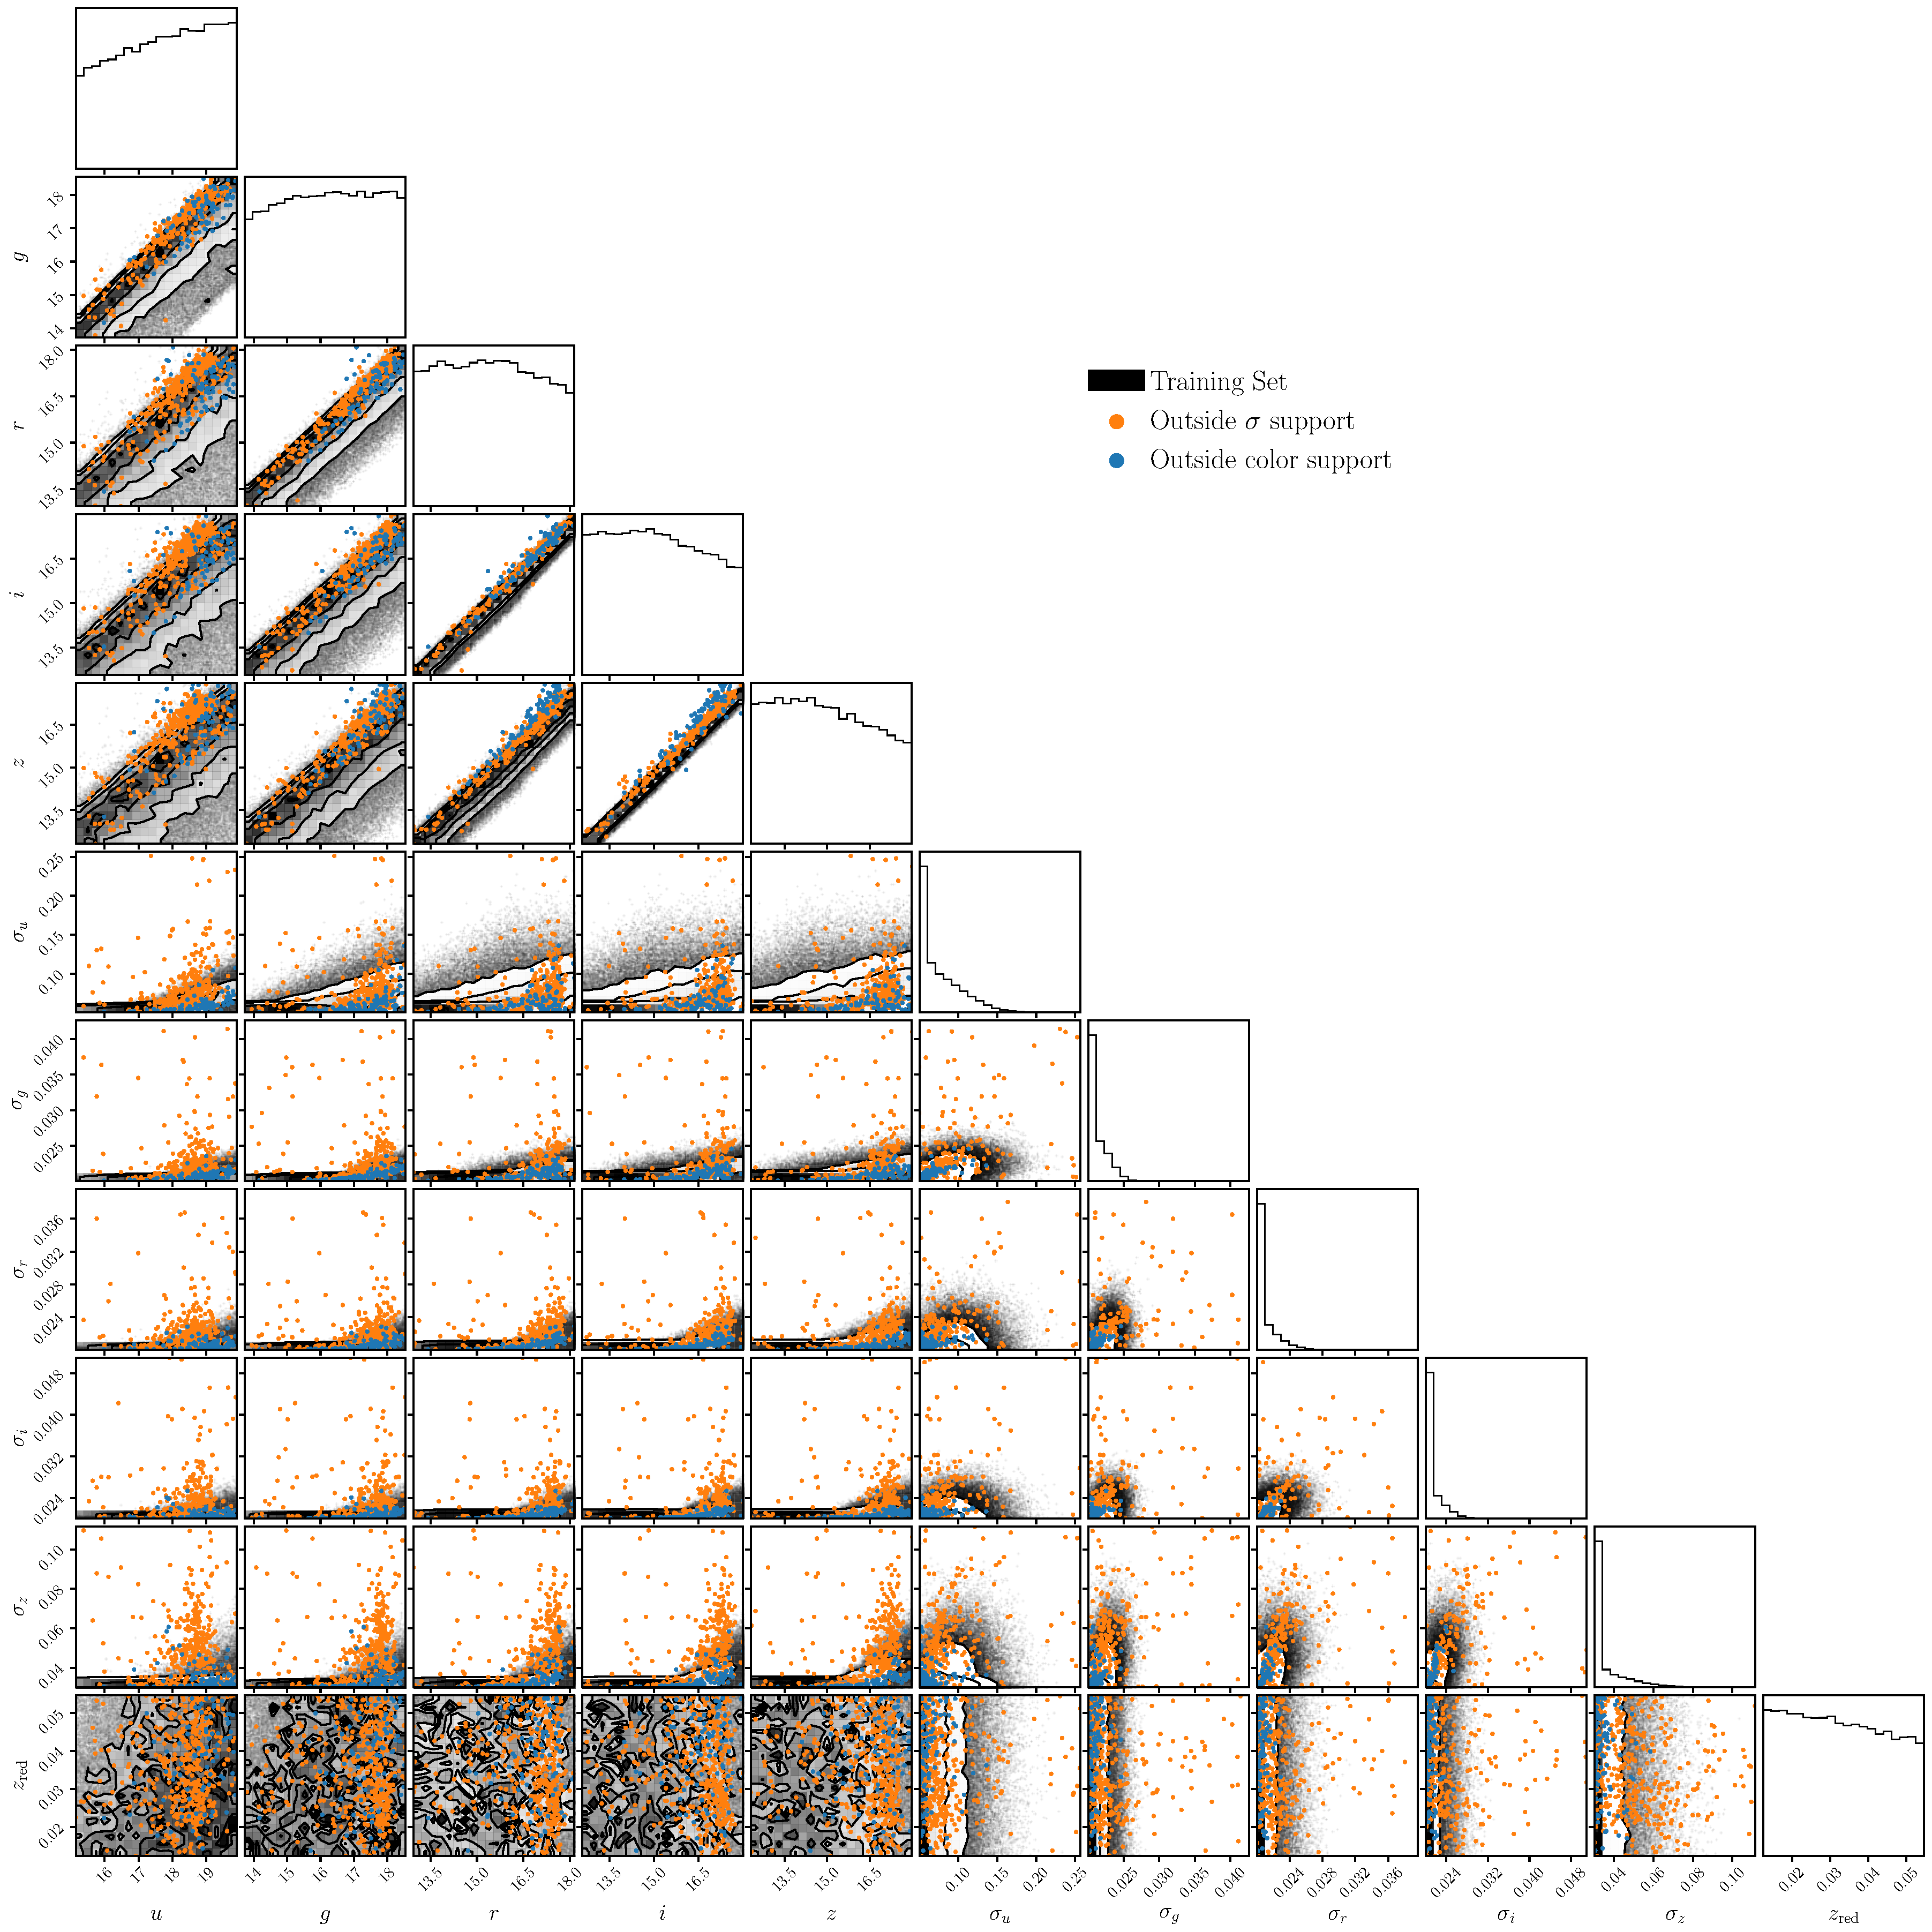
\includegraphics[width=0.9\textwidth]{figs/fails.pdf}
    \caption{\label{fig:fail}
    The distribution of photometric magnitudes, uncertainities, and redshift of
    NSA galaxies for which \sedflow~does not produce valid posteriors. 
    These galaxies lie outside of the suport of the \sedflow~training data
    (black) so \sedflow~cannot accurately estimate their posteriors. 
    We mark the NSA galaxies that have unusually high photometric uncertainties
    that are not accounted for in our noise model in orange and galaxies that
    have photometric colors that cannot be modeled by our SED model in blue. 
    }
\end{center}
\end{figure}
% paragraph discussing photometric uncertainty outliers
We classify NSA galaxies as (1) in Figure~\ref{fig:fail}, if they have
$\sigma_X$ that is unusually high for a given $f_X$ in at least one photometric
band: $\sigma_X > \mu_{\sigma_X}(f_X) + 3 \sigma_{\sigma_X}(f_X)$
(see Eq.~\ref{eq:noise}). 
There are 490 NSA galaxies without valid \sedflow~posteriors due to (1).
These galaxies have a $\bfi{x}$ distribution that is significant discrepant
from the distribution of the training data, with many galaxies that lie well
beyond the locus of training data points. 
The \sedflow~estimate of $p(\btheta \given f_X, \sigma_X, z)$ is only accurate in
regions of $\bfi{x}$-space where there is sufficient training data. 
This requirement is not met for these NSA galaxies.  
In principle, if we use a more conservative noise model than Eq.~\ref{eq:noise}
and construct noisier training data, we can expand the support of \sedflow. 
\sedflow~would then produce sensible posteriors for more NSA galaxies. 
However, there is an inherent trade-off. 
For a training data set of fixed size, a more conservative noise model would
reduce the amount of training data in $\bfi{x}$-space where the vast majority
of NSA galaxies lie and can reduce the accuracy of the posteriors in these
regions. 
Since, \sedflow~fails for only a small fraction of NSA galaxies, we do not
explore more conserative noise models in this work.

% paragraph discussing color outliers
Next, we examine the NSA galaxies that lie outside of the \sedflow~support
because they have colors that cannot be modeled by our SED model. 
In Figure~\ref{fig:fail}, we classify NSA galaxies as (2) if any of their
colors (\emph{e.g.} $u-r$, $u-g$, $r-z$) is bluer than the 99.9\% percentile of
the training data color. 
There are 98 NSA galaxies without valid \sedflow~posteriors due to (2).
The $i$ versus $z$ magnitude panel in particular highlights how a significant
number of NSA galaxies are bluer than the training data. 
The fact that the training data do not span these colors suggests that the
PROVABGS SED model may not fully describe all types of galaxies in observations. 
As we discuss in Section~\ref{sec:discuss}, this may be due to limitations in
the SFH and ZH prescription in the PROVABGS model or even in our understanding
of stellar evolution. 
Limitations of the SED model equally impacts conventional MCMC sampling
approaches and is beyond the scope of this work. 
We, therefore, do not examine the issue further. 
For completeness, we derive posteriors for NSA galaxies for which \sedflow~fails
to estimate valid posteriors using PROVABGS with MCMC sampling with the same
configuration as \cite{hahn2022}. 

%\bibliographystyle{mnras}
\bibliography{sedflow} 
\end{document}
